\section{Absicherung}

\subsection{Architektur und Design}

\subsection{LISP Map Server}
Es gibt zwei Betriebsarten für einen LISP Map-Server(MS): 
\begin{itemize}
	\item als Map-Resolver(MR), der Map-Requests von einem ITR entgegennimmt und das EID-zu-RLOC-Mapping mit Hilfe der verteilten Mapping-Datenbank auflöst
	\item als Map-Server(MS), der autoritative EID-zu-RLOC-Mappings von einem ETR lernt und in der Datenbank veröffentlicht
\end{itemize}

Zur Bereitstellung gibt es zwei Varianten. Zum einem kann es einen redundanten globalen MSMR geben, oder es werden pro Fabric ein MSMR implementiert.

\subsubsection{Redundante MS / MR Bereitstellung}

Es wird empfohlen, redundante Standalone MS- und MR-Systeme mit den MS / MR-Funktionen auf demselben Gerät bereitzustellen. Wenn redundante eigenständige MS / MR implementiert werden, müssen sich alle xTRs bei beiden MS registrieren, so dass jeder eine konsistente Sicht auf den registrierten LISP EID-Namespace hat. Für Map-Resolver-Funktionalität ist die Verwendung einer Anycast-IP-Adresse wünschenswert, da dadurch die Mapping-Lookup-Leistung verbessert wird, indem der MR ausgewählt wird, der dem anfordernden ITR am nächsten ist.

\begin{figure}[H]
	\centering
	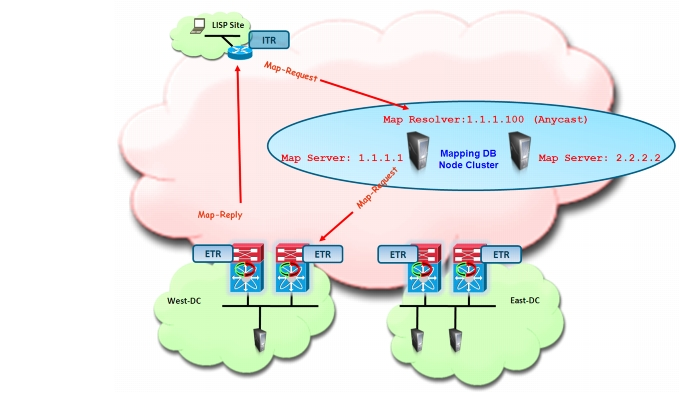
\includegraphics[width=1\linewidth]{img/Analyse/LISP-Example}
	\caption{Redundante MS / MR Bereitstellung \cite{LISP-mobility} }
	\label{fig:Redundante MS / MR Bereitstellung}
\end{figure}

\subsubsection{Co-Lokalisierung von MS / MR und xTR Funktionalitäten}

Ein weiteres Beispiel ist die Co-Lokalisierung  von MS / MR- und xTR-Funktionalitäten. Das co-lokalisierte Modell ist besonders vorteilhaft, da es die Gesamtzahl verwalteter Geräte reduziert, die zum Ausrollen einer LISP Host Mobility-Lösung erforderlich sind. 

Die erforderliche Konfiguration würde aber in beiden Szenarien identisch bleiben, indem eindeutige IP-Adressen genutzt werden, um die Map-Server und eine Anycast-IP-Adresse für den Map-Resolver zu identifizieren.

\begin{figure}[H]
	\centering
	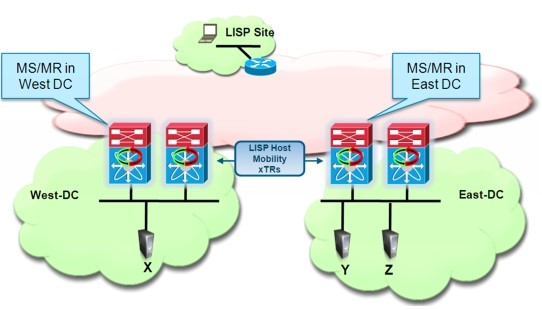
\includegraphics[width=0.8\linewidth]{img/Analyse/LISP-Example2}
	\caption{Co-Lokalisierung von MS / MR und xTR Funktionalitaeten \cite{LISP-mobility} }
	\label{fig:Co-Lokalisierung von MS / MR und xTR Funktionalitaeten}
\end{figure}

Es kann also ein redundantes eigenständiges MS / MR-Modell bereitgestellt werden, indem dedizierte Systeme zur Durchführung dieser Mapping-Funktionen genutzt werden (siehe Abbildung 2.9) oder alternativ können die MS- und MR-Funktionen gleichzeitig auf dem Netzwerkgerät, welches bereits die xTR-Rolle ausführt, implementiert werden (siehe Abbildung 2.10).

\subsubsection{Anwendung}
Damit bei einem Ausfall eines MSMR nicht alle Fabrics betroffen sind, macht es Sinn pro Fabric einen redundanten MSMR zu implementieren. So können auf einem xTR eine oder mehrere MSMR-Adressen konfiguriert werden.

Abfragen, die ein EID-zu-RLOC-Mapping durchführen, sind datengesteuert. Dieses Verhalten bedeutet, dass ein neuer Datentransfer zwischen LISP-Sites ein Mapping-Lookup erfordert, was dazu führt, dass der Datenversand wird gestoppt, bis ein Mapping durchgeführt wurde. Dies Verhalten ist analog zum DNS-Protokoll und ermöglicht LISP die folgenden Funktionen in einer dezentralen Datenbank mit EID-zu-RLOC-Mappings zu betreiben. 

Die Replikation der gesamten (potenziell umfangreichen) Datenbank ist unnötig, da auf Mappings bei Bedarf zugegriffen wird, genau wie im DNS muss ein Host nicht die komplette Domänendatenbank kennen. Tunnelrouter verwalten den Map-Cache der zuletzt verwendeten Mappings, um die Leistung des Systems zu verbessern.

\paragraph{LISP Client Registration}
Wird ein noch unbekannter neuer Client an die Fabric angeschlossen, sendet der ITR einen Map-Request an einen bekannten MR, wenn es ein EID-zu-RLOC-Mapping benötigt, das noch nicht in seinem lokalen Map-Cache vorhanden ist.

\begin{figure}[H]
	\centering
	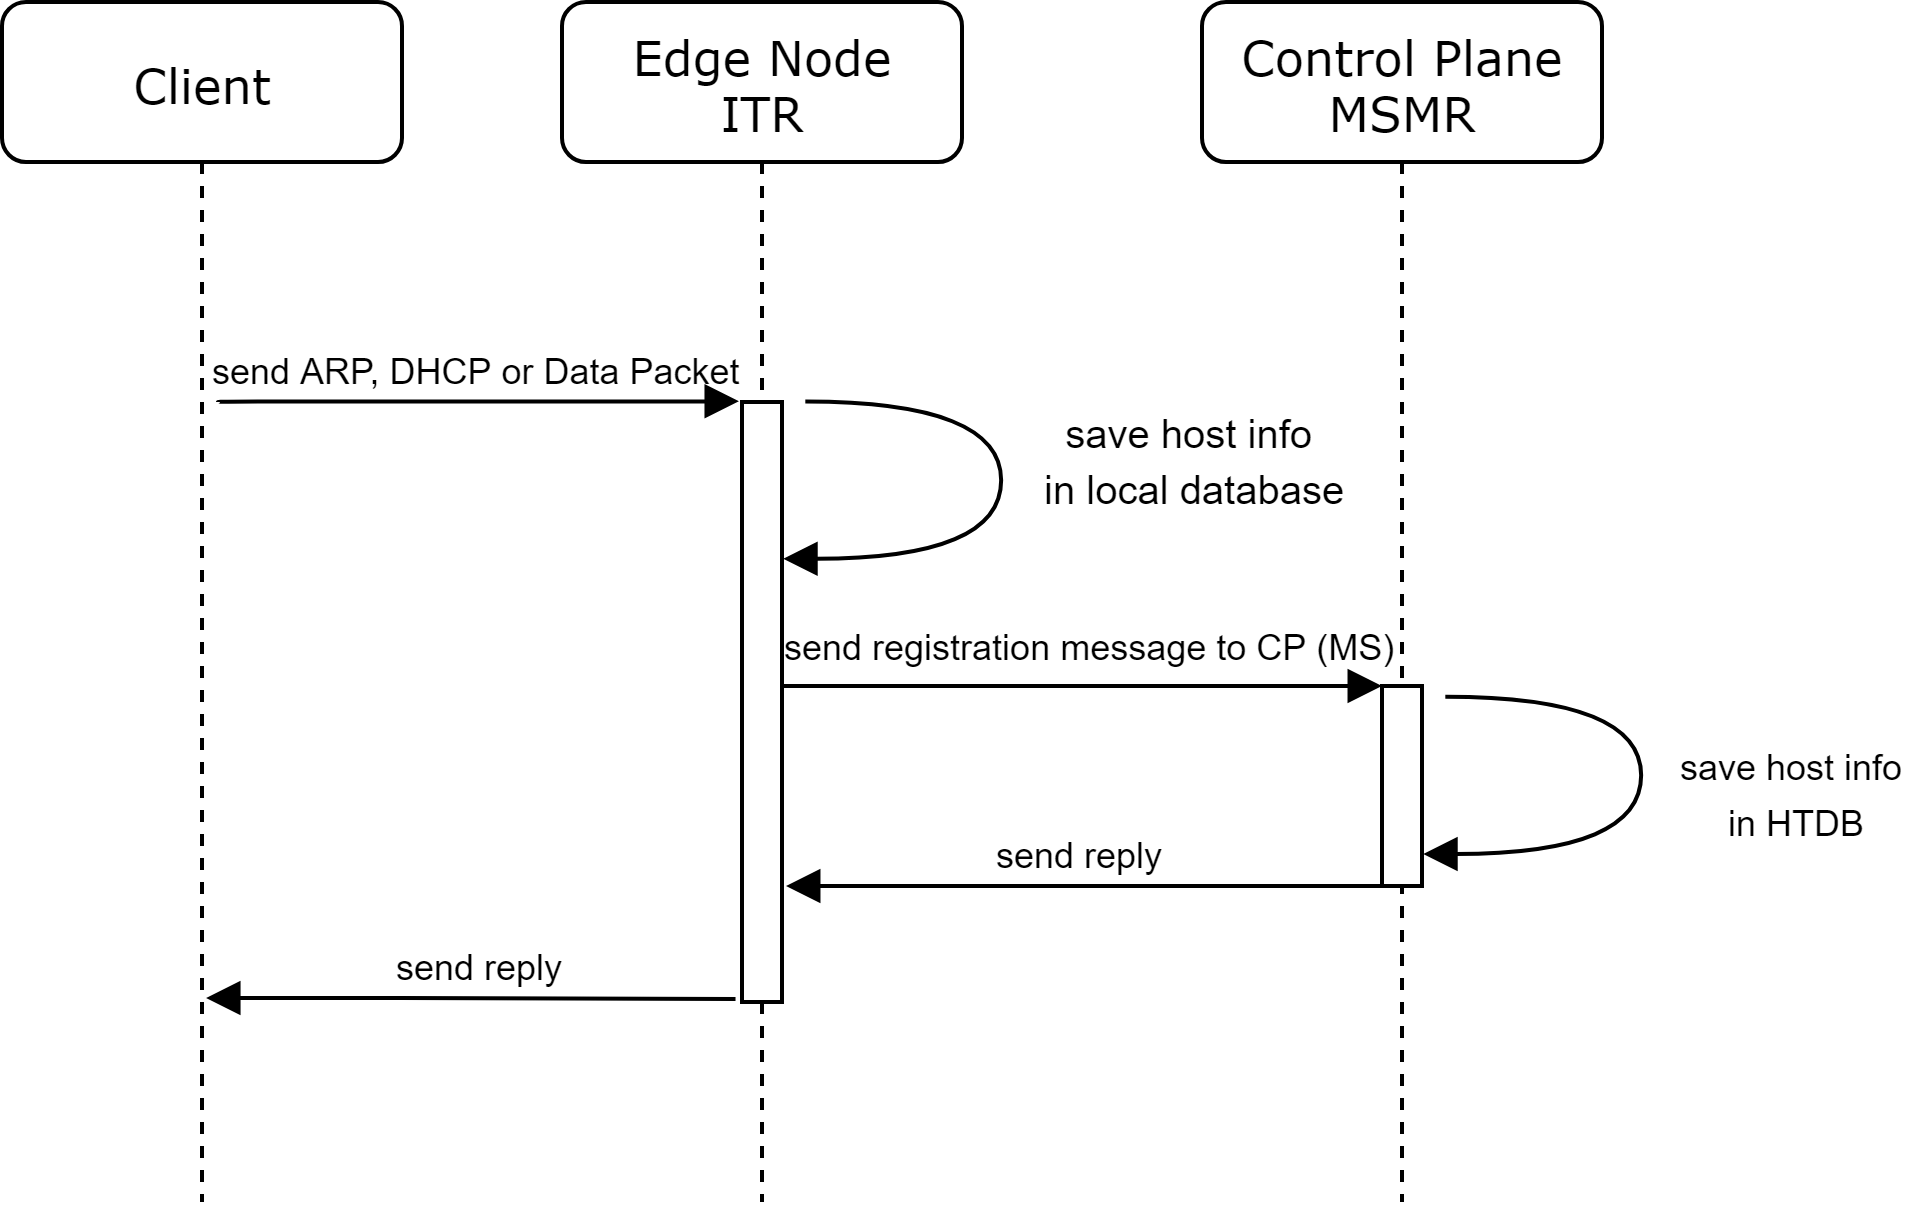
\includegraphics[width=0.8\linewidth]{img/Absicherung/LISP-ClientRegistration}
	\caption{LISP Client Registration}
	\label{fig:LISP Client Registration}
\end{figure}

\paragraph{LISP Host Resolution}
Will ein Client mit einem noch unbekannten anderen Client kommunizieren, so sucht sein ITR zuerst in seinem lokalen Map-Cache nach einem Eintrag. Ist noch kein Eintrag zum Client2 vorhanden, so schickt der ITR ein Map-Request zu seinem MR. Der MS sendet dann den originalen Map-Reguest an den zuletzt registrierten ETR. Da Client2 noch am ETR angeschlossen ist, sendet dieser einen Map-Reply an den ITR, welcher die angefragten Mapping-Informationen enthält.

Bei einem Ping werden die initialen Pakete verworfen, bis die Host Resolution abgeschlossen ist. 

\begin{figure}[H]
	\centering
	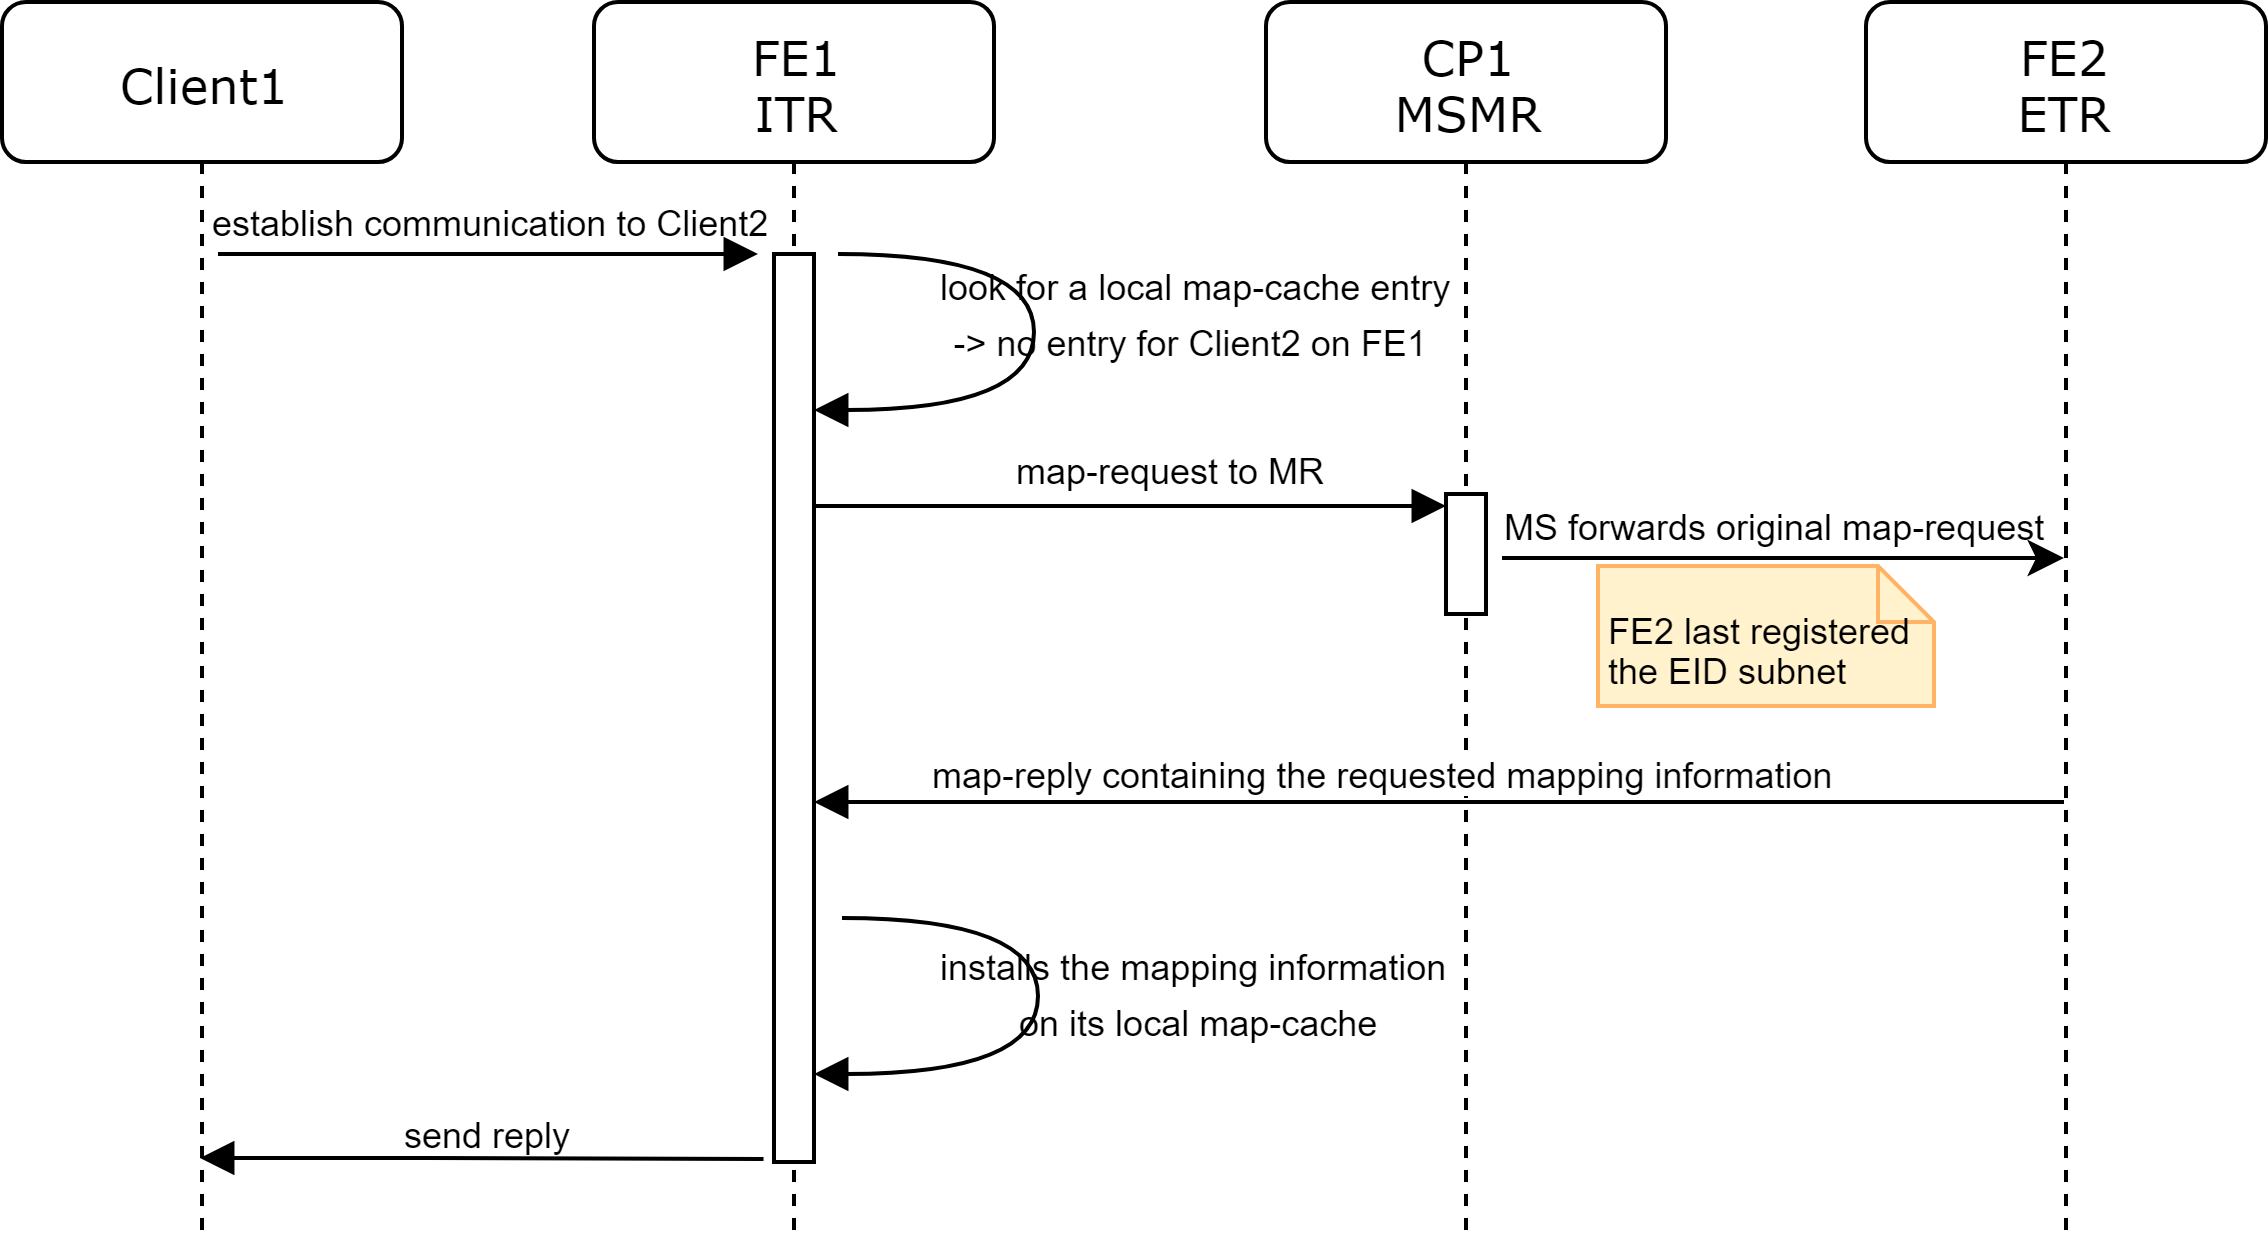
\includegraphics[width=1\linewidth]{img/Absicherung/LISP-HostResolution}
	\caption{LISP Host Resolution}
	\label{fig:LISP Host Resolution}
\end{figure}

\paragraph{Host Mobility}
Die Host Mobility ist ähnlich wie die Client Registration, da der Client sich beim neuen FE2 zuerst registriert und die neuen Informationen schliesslich vom CP1 dann an den alten FE1 zur Aktualisierung weitergegeben werden.

\begin{figure}[H]
	\centering
	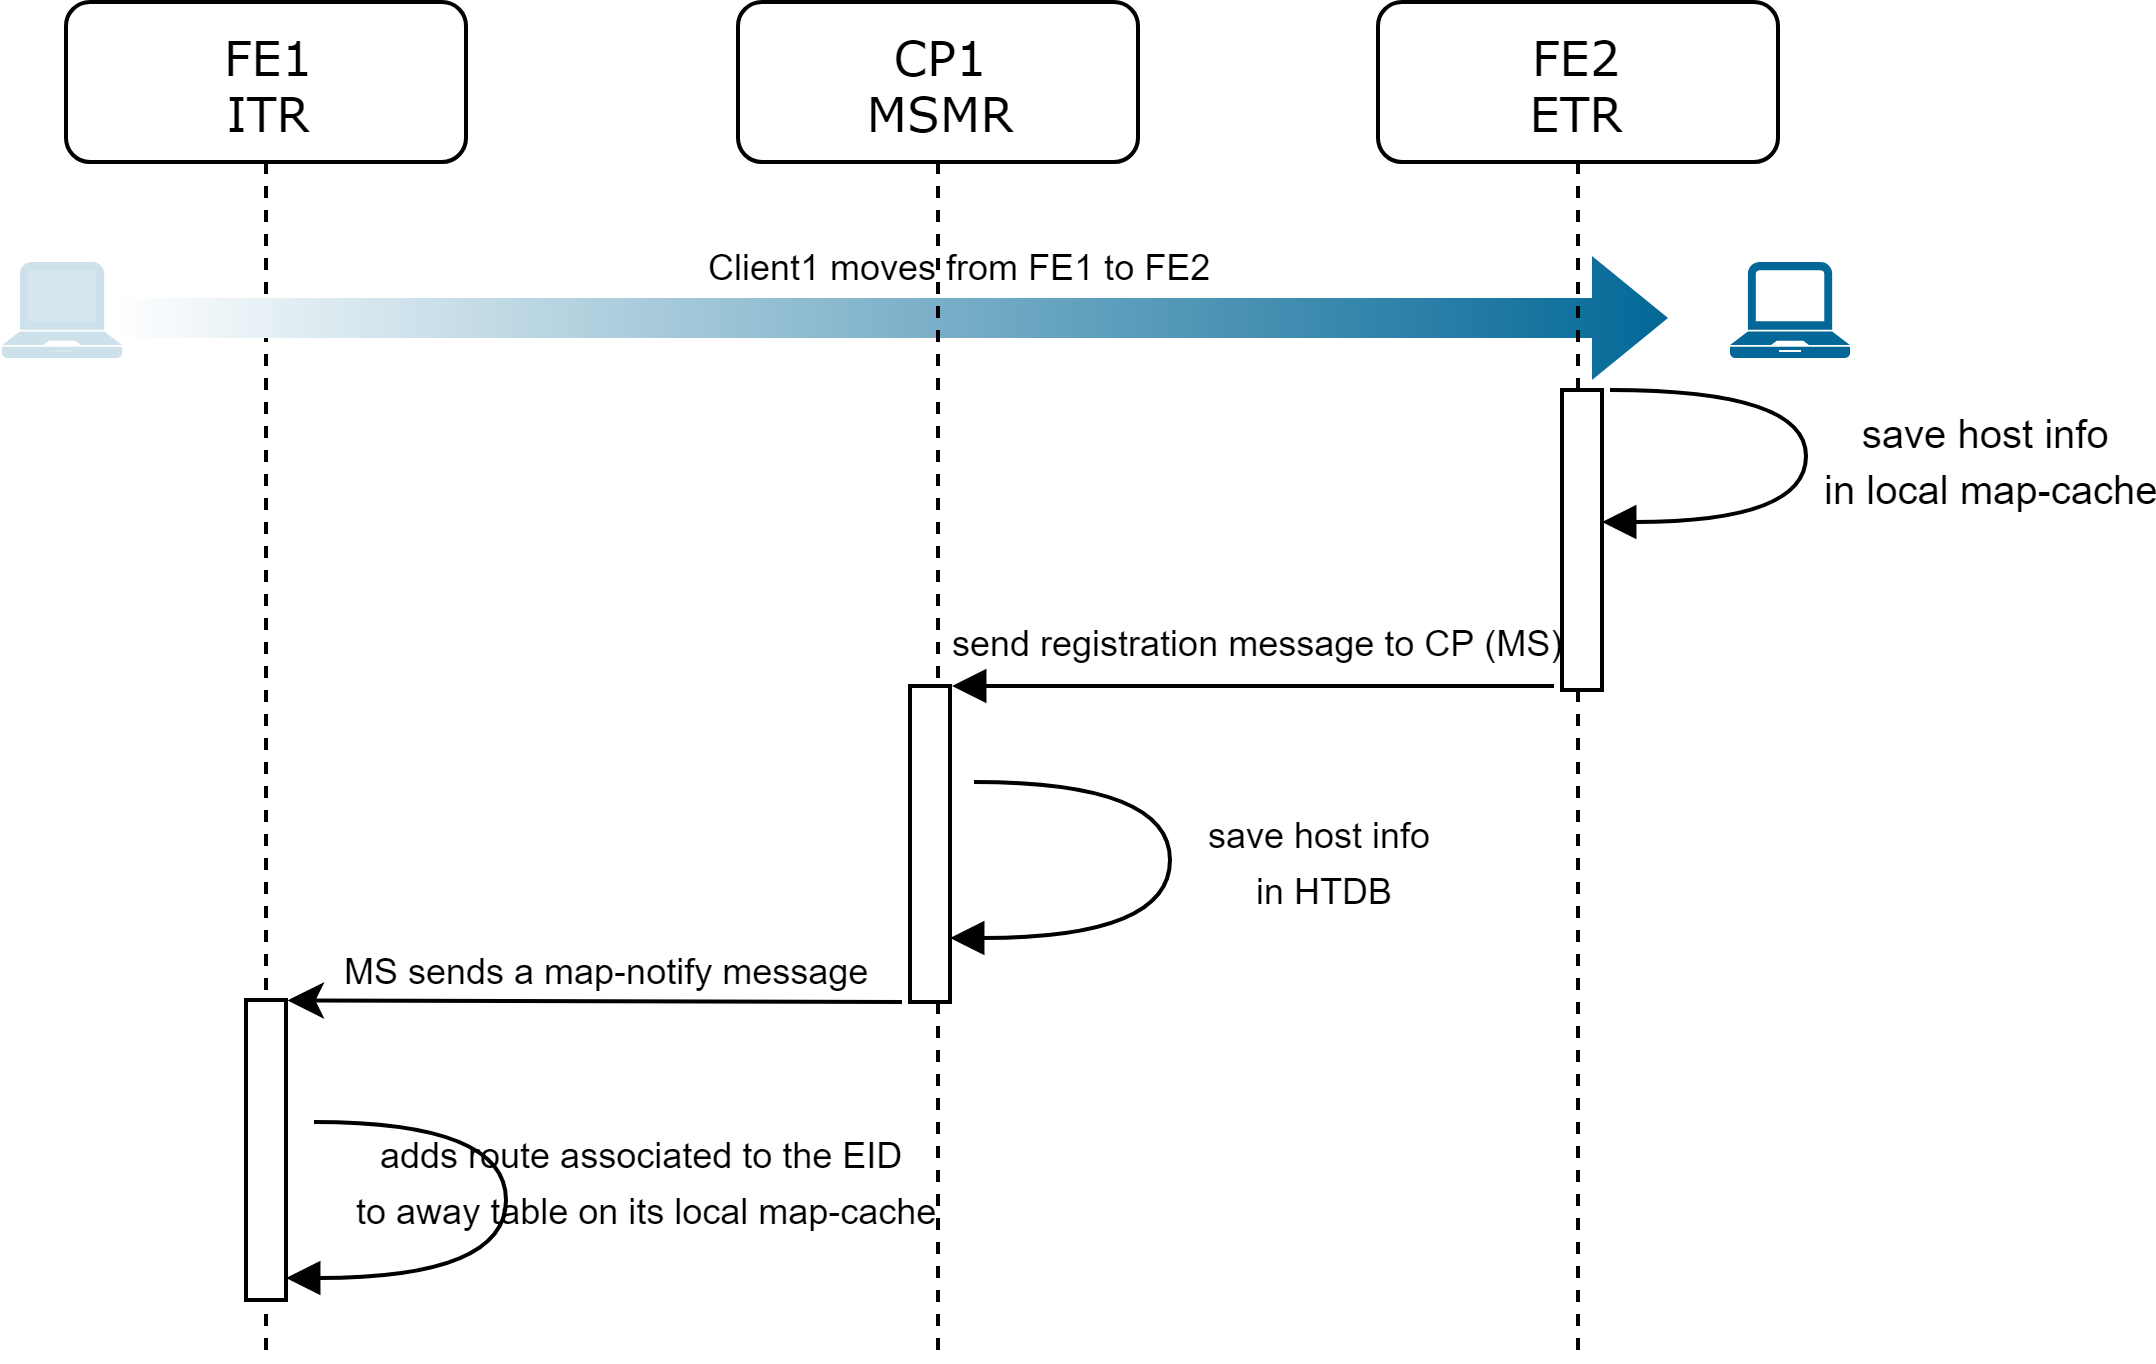
\includegraphics[width=1\linewidth]{img/Absicherung/LISP-HostMobility}
	\caption{LISP Host Mobility}
	\label{fig:LISP Host Mobility}
\end{figure}

Wenn ein dynamischer EID zwischen Rechenzentrumsstandorten wechselt, müssen die lokalen LISP Host Mobility-xTRs ihre Existenz erkennen. 

Das für LISP Host Mobility konfigurierte LISP xTR erkennt ein neues dynamisches EID-Verschiebungsereignis, wenn:

\begin{itemize}
	\item 
\end{itemize}

\subsubsection{Ausfall MSMR}
Bei einem Ausfall des MSMR kann keine Host Registration mehr vorgenommen werden. Das heisst neue Clients können keine Verbindung zum restlichen Netzwerk aufbauen. Bestehende Clients können nur mit Clients welche am selben FE angeschlossen sind kommunizieren. Dies jedoch nur solange ihr Eintrag im lokalen Map-Cache bestehen bleibt. Der TTL der Einträge im Map-Cache beträgt per default einen Tag. 

Da jeder xTR seinen eigenen Map-Cache hat und kann sich sein Inhalt innerhalb derselbe LISP-Site unterscheiden. Daher können xTr leicht schwere Paketausfälle erleiden und mit LISP Control Messages geflutet werden.  

\subsection{ISE / Radius}

\subsection{SGT Access List}

\subsection{Border Node}

\subsection{Fusion Router}

\subsection{DHCP}

\subsection{DNS}

\subsubsection{Infoblox HA Cluster}


\subsubsection{Read Only DNS Server an Aussenstandorten}
	
Damit Aussenstellen nicht auf DNS Server des Hauptstandortes angewiesen sind, kann in jedem Standort ein Read-Only Server betrieben werden. Somit funktioniert die Namensauflösung auch im Falle eines Kommunikationsverlusts zum Hauptstandort. 

\begin{figure}[H]
	\centering
	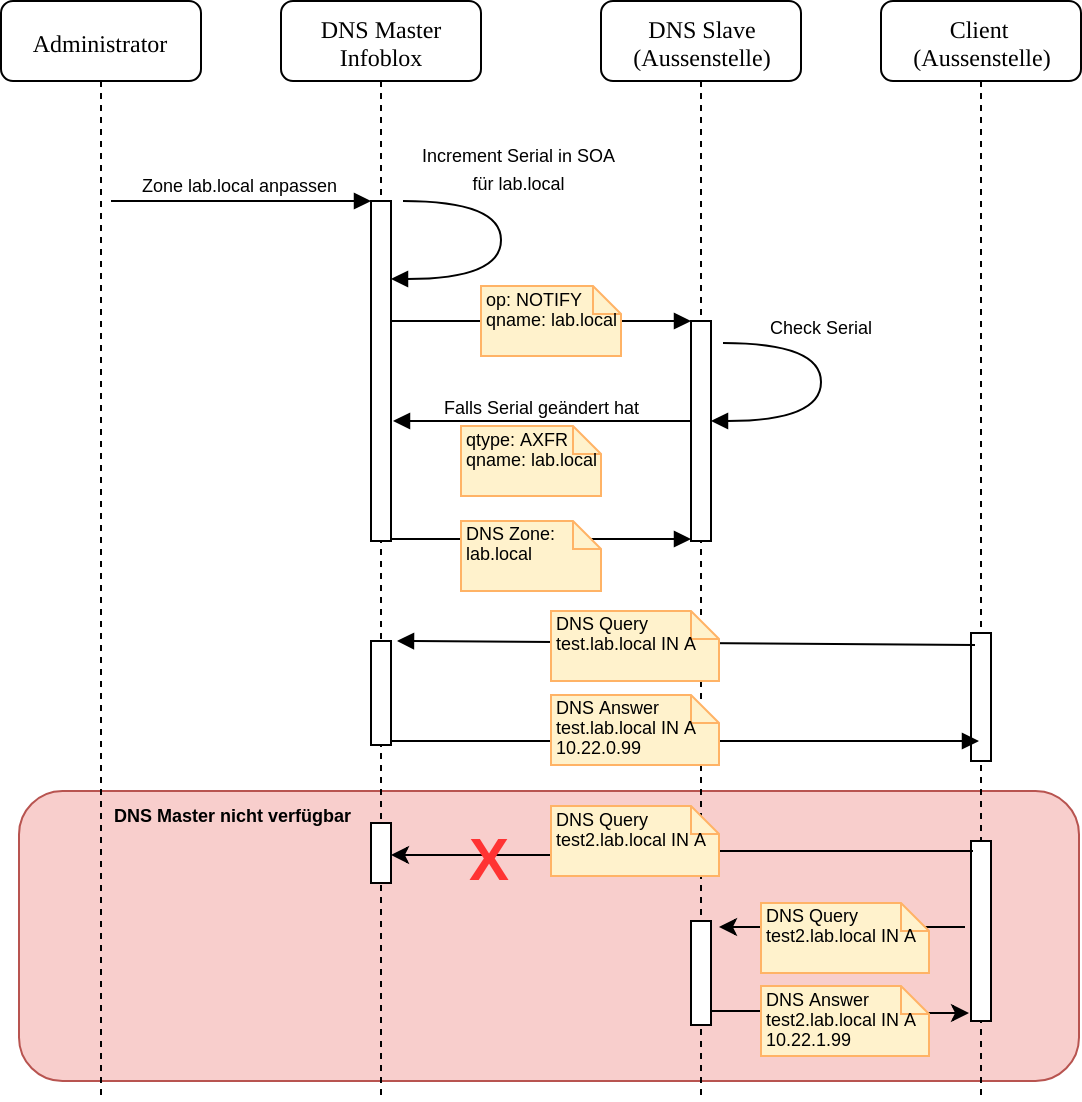
\includegraphics[width=0.8\linewidth]{img/Absicherung/DNS_Sequenzdiagram.png}
	\caption{DNS Sequenzdiagramm}
	\label{fig:DNS Sequenzdiagramm}
\end{figure}
\paragraph{Infoblox}

Damit die Read-Only Server stets über die aktuellsten DNS Zonen verfügen, müssen die Informationen von Infoblox auf diese repliziert werden. In diesem Fall wird dafür der Zone Transfer verwendet. Dazu muss dies in Infoblox für alle Slave Server erlaubt werden. 

Dies wird in Infoblox via \textit{Grid $\rightarrow$ DNS $\rightarrow$ Infoblox Instanz $\rightarrow$ Edit $\rightarrow$ Zone Transfers} ausgeführt.

\begin{figure}[H]
	\centering
	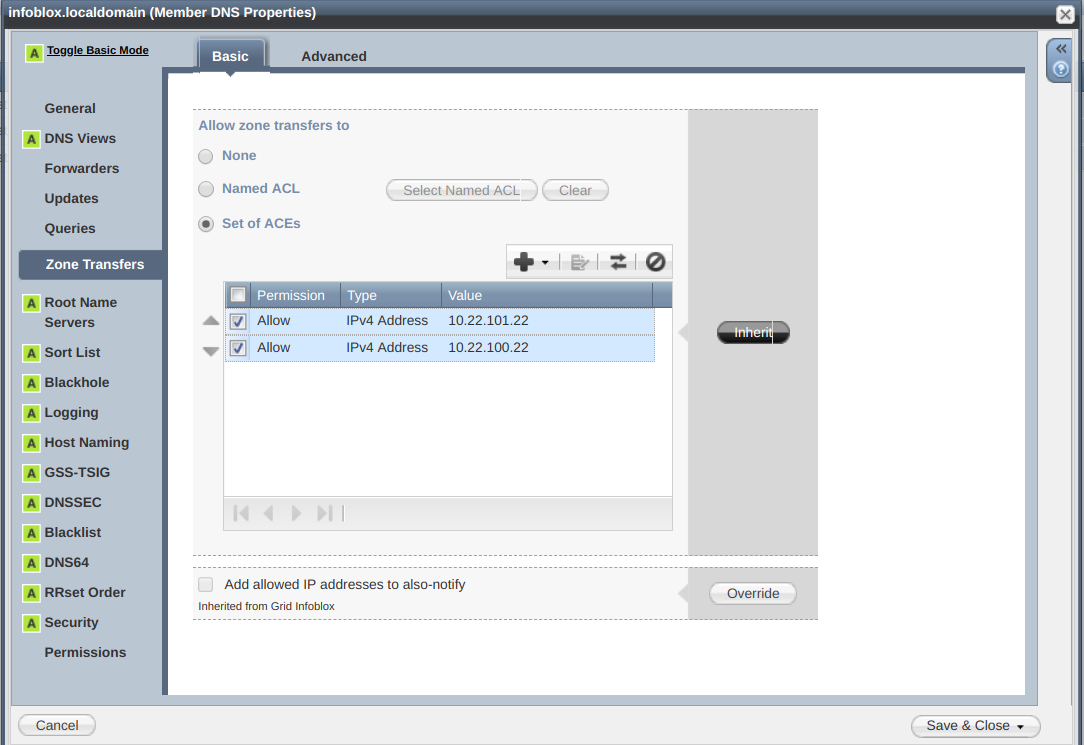
\includegraphics[width=0.8\linewidth]{img/Absicherung/Infoblox_Zone_Transfer.png}
	\caption{Infoblox Zone Transfer}
	\label{fig:Infoblox Zone Transfer}
\end{figure}

\paragraph{DNS Slaves}

Auf den Slaves an den jeweiligen Aussenstandorten müssen die Zonen als Slave Zonen konfiguriert sein und Infoblox muss als Master konfiguriert werden. Dadurch können die Zonen vom Master auf den Slave transferiert werden. Der Slave aktualisiert alle Slave Zonen in regelmässigen Abständen. Dieser Intervall wird in der Zone im SOA Record mit dem "Refresh" Parameter definiert.
Zusätzlich kann auf dem Master konfiguriert werden, dass alle Slaves mittels "Notify" informiert werden, sobald sich eine Zone ändert, worauf der Slave die aktuellsten Informationen für diese Zone abruft. Somit ist sichergestellt, dass alle Server an Aussenstandorten stets über eine aktuelle Konfiguration verfügen.

\paragraph{Clients}

Auf den Cliens ist es wichtig, dass alle nötigen DNS Server in der korrekten Reihenfolge konfiguriert werden. Als erster Server soll der Master, also Infoblox eingetragen werden. Sofern Infoblox als Cluster betrieben wird, können auch alle Instanzen des Clusters verwendet werden. Danach der Slave am jeweiligen Standort. Dies sorgt dafür, dass der Slave nur dann verwendet wird, wenn die Kommunikation zum Master nicht funktioniert.